\documentclass[conference]{IEEEtran}
\usepackage{amsfonts}
\usepackage{mathrsfs}
\usepackage{amsthm,amssymb,amscd,amsmath}
\usepackage{tikz}
% 图形相关依赖
\usepackage{graphicx}
\usepackage{float}

% ===== 加宽双栏、缩小栏间距 开始 =====
\setlength{\columnsep}{20pt}   % 原来默认约20pt，改10-15pt都可以
\setlength{\textheight}{24cm}
\setlength{\textwidth}{18.5cm}
% ===== 加宽双栏、缩小栏间距 结束 =====

\newtheorem{thm}{Theorem}[section]
\newtheorem{lem}[thm]{Lemma}
\newtheorem{con}[thm]{Conjecture}
\newtheorem{cor}[thm]{Corollary}
\newtheorem{defi}[thm]{Definition}
\newtheorem{rem}[thm]{Remark}
\newtheorem{exam}[thm]{Example}
\newtheorem{prop}[thm]{Proposition}

\begin{document}

\title{OADM: Optimally Approximate Floating-Point Divider-Multiplier with Runtime Configurability\footnote{Project partially supported by the National Natural Science Foundation of China (No.)}}
%\author{
%\IEEEauthorblockN{Pingchuan Dong and Cheng Zhuo}
%\IEEEauthorblockA{New York University\\Zhejiang University\\Key Laboratory of Collaborative Sensing and Autonomous Unmanned %Systems of Zhejiang}
%}
\maketitle

\begin{abstract}
Approximate computing is a promising alternative to improve energy efficiency for IoT devices on the edge. By use of tangent planes, this work mainly proposes an optimally approximated floating-point divider with runtime configurability. We turn the division approximation to an optimal problem and obtain a theoretically sound formula, which is similar to the formula of the approximated floating-point multiplier in \cite{CTChen}. With the approximate formula, a multi-level architecture is proposed to implement the run-time configurability and the proposed divider strikes an advantageous balance between accuracy and resource efficiency comparing to the prior state-of-the-art approximate dividers. Furthermore inspired by the similarities observed in \cite{CTChen}, we propose a unified hardware architecture supporting both approximate floating-point division and multiplication. The proposed unified divide-multiply unit can be configured to execute either approximate division or approximate multiplication in circuit with simple logic operations.
\end{abstract}

\begin{IEEEkeywords}
tangent plane, approximate computation, divider, multiplier
\end{IEEEkeywords}

\section{INTRODUCTION}
\label{Intro1}
Energy efficiency has emerged as one of most critical criteria in computing systems design in recent years.
Though in general computing systems are designed to generate accurate outputs,  applications in domains of computer vision and machine learning can tolerate amounts of inaccuracies in their computations. Computational accuracy is traded for reductions in power consumption and design complexity \cite{JHan} \cite{VGupta2011}.

In approximate hardware design, hardware elements are simplified to reduce the power consumption and design area, therefore adding inaccuracies. The implementation of these approximations are mostly focused on basic arithmetic building blocks (e.g. adders and multiplier), due to their high utilization in different applications. These
approximate designs can then replace or augment their accurate counterparts in general purpose processors.

While a number of designs for approximate adders and multipliers have been proposed, the approximate design of dividers
is not as well investigated. Arithmetic divider is a basic yet complex module in integrated circuits. It plays an increasingly important role in a
variety of fields and is widely used in graphic processing. However, divider is often a performance limiting module in
these applications due to its complexity. The lack of fast division module in integrated circuits has for a long time been the bottleneck for some real-time multimedia applications. This work aims to address this issue, by proposing OADM (an {\bf O}ptimally {\bf A}pproximated Floating-Point {\bf D}ivider-{\bf M}ultiplier).
Our main contributions are as follows:

\begin{itemize}
\item By use of tangent planes, an optimization formulation is given to optimize the error of the approximate divider which acts as the basis of the divider architecture; furthermore, we modify the proposed formula and obtain a new formulation with unbiased  error distribution.
\item Based on the optimization formulation mentioned above, we present a novel multi-level approximate FP divider with run-time configurability. To enhance the accuracy, we can add up the error compensations of increasing levels from the level 0. The circuit for the error compensation of each level is easily implemented with shift, inversion and substraction. This reduce the cost complexity from exponential to linear function of levels $n$ directly.
\item For different levels, we derive mathematical formulation for the absolute error of approximations in the proposed divider by the Taylor's Theorem for two variables.
\end{itemize}

The experimental results clearly demonstrate that, in comparison to state-of-the-art dividers, OADM strikes an advantageous balance between accuracy and resource efficiency.
{\bf (In this paragraph, we should list the experimental results simply. Read \cite{CWen} for reference )}

The rest of the paper is organized as follows. In Section \ref{PreviousWork2}, we review some previous related works on the approximated arithmetics; in Section \ref{AppDivider3}, we propose the design of approximated divider architecture and give the analytical error analysis in Section \ref{ErrAna4}; in Section \ref{Experiment5} and Section \ref{Application6}, we evaluate the performance of the proposed approximate divider with experimental results and in real applications; finally, we summarize our conclusion in Section \ref{Conlusion7}.

\section{PREVIOUS WORK}
\label{PreviousWork2}
In this section, we review some of the related prior work done in the area of approximate design. Approximate architecture can enable the designer to introduce inaccuracies in a controlled and deterministic manner.

While a few approximate designs have been proposed for both adders and multipliers \cite{VGupta2013,SHashemi2015,HMahdiani2010,CTChen}, dividers and other arithmetic units have
not received as much attention. This is due in part to lower utilization of blocks such as dividers compared to adders and multipliers and
the main reason of the lower utilization of dividers is in part a result of high cost of dividers in terms
of delay and power. As shown in \cite{HSaadat1}, an accurate FP divider incurs more than 15$\times$ Area-Delay-Product and over 1.5$\times$ power consumption
compared to an accurate FP multiplier. Therefore, approximate divider design with significant improvements in these areas can facilitate utilization of
these arithmetic blocks.

Recently, several works on approximate dividers have been proposed. These methods have their own advantages, disadvantages and mainly focus on:
\\
(1) truncation-based \cite{LChen,SHashemi3,HJiang9}. The ideas lie on dynamically select the most relevant bits of each of the operands and reduce complexity by discarding the lower, less significant bits. Truncated-based designs can achieve high computational accuracy, but often need  a smaller accurate divider design in its core and so impose substantial
hardware overhead;\\
(2) logarithm-based \cite{HSaadat1,MImani4,OGRatnaparkhi5}. These designs depend on the approximation $\log_{2}(1+a)\approx a$ mainly. Since the error of the approximation $\log_{2}(1+a)\approx a$ is small only if $a$ is close to zero, logarithm-based designs are more hardware-efficient but should balance between the two accuracy and configurability during runtime;\\
(3) reciprocal-based dividers \cite{JMelchert2,JOelund6,Bhargav,CWen,HLiu}. These dividers use different ways to approximate the reciprocal
${1\over y}$ of divisor $y$, such as Taylor's expansions\cite{JMelchert2}, Newton Raphson method\cite{Bhargav}, quadratic curve fitting\cite{HLiu} and piece-wise linear segments\cite{CWen};\\
(4) In \cite{LWu15}, the proposed approach is based on the curve fitting method to approximate the curved surfaces with small square planes as follows:
$${x\over y}\approx p\cdot x-q\cdot y+r.$$
First decide the partition scheme and then use the Matlab curve-fitting toolbox to find the coefficients $p, q$ and $r$ for the
square/triangular plane to approximate the individual region of the curved surfaces ${x\over y}$. The Look-up Table stores the coefficients
$p, q$ and $r$. Since there are no concrete information about the constants $p, q, r$,  the proposed architecture relies on pre-loaded lookup tables (LUTs), making runtime adjustments to accuracy impossible.

\section{PROPOSED APPROXIMATE FP DIVIDER-MULTIPLIER}
\label{AppDivider3}
Comparing to integer computing, FP arithmetic is more complex and so energy consuming. According to IEEE 754 standard in \cite{Ieee}, an FP number $F_{x} $ consists of
sign, mantissa and exponent as follows:
\[F_{x}=sign_{x}\times x\times 2^{E_{x}},\;\forall x\in [1, 2)\]
where $sign_{x}, x, E_{x}$ refer to the sign, mantissa and exponent of $F_{x}$ respectively. Thus for two FP numbers $F_{x}$ and $F_{y}$, the division is:
$${F_{x}\over F_{y}}=sign_{x}sign_{y}\times {x\over y}\times 2^{E_{x}-E_{y}}.$$
In a general processor, for an FP division, the sign bits is computed by an XOR operation and the exponent bits are computed by a subtractor. The division ${x\over y}$ of two mantissas is much more energy consuming and costlier than the computations of signs and exponents. The motivation of this work is to propose an energy efficient divider for ${x\over y}$ between mantissas.

\subsection{First Method}
\label{First3.1}
On $[y_{1}, y_{2}]$, our aim is to approximate $f(y)={1\over y}$ by the tangent line $g(y)=-{y\over p^{2}}+{2\over p}$ of some point $p$ in $[y_{1}, y_{2}]$. We try to find
a point $p$ which minimizes the error function
\begin{eqnarray}
E_{I}(p)&=&\int_{y_{1}}^{y_{2}}[{1\over y}-(-{y\over p^{2}}+{2\over p})]dy\nonumber\\
&=&\ln y_{2}-\ln y_{1}+{y_{2}^{2}-y_{1}^{2}\over 2p^{2}}-{2\over p}(y_{2}-y_{1}).\nonumber
\end{eqnarray}
By $$0=E_{I}'(p)=(y_{1}^{2}-y_{2}^{2})p^{-3}+2(y_{2}-y_{1})p^{-2},$$
we obtain $p={y_{1}+y_{2}\over 2}$. Following the symbols in \cite{CTChen}, we let $k_{1}={y_{1}+y_{2}\over 2}, k_{2}={x_{1}+x_{2}\over 2}$. Thus on $[x_{1}, x_{2}]\times [y_{1}, y_{2}]$,
we have
\begin{eqnarray}
{x\over y}=x\cdot{1\over y}&\approx&x\cdot(-{y\over k_{1}^{2}}+{2\over k_{1}})\nonumber\\
&=&-{1\over k_{1}^{2}}xy+{2\over k_{1}}x\nonumber\\
&\approx&-{1\over k_{1}^{2}}(-k_{1}k_{2}+k_{1}x+k_{2}y)+{2\over k_{1}}x\nonumber\\
&=&-{1\over k_{1}^{2}}(-k_{1}k_{2}+k_{1}x+k_{2}y-2k_{1}x)\nonumber\\
&=&{1\over k_{1}^{2}}(k_{1}k_{2}+k_{1}x-k_{2}y),\label{FirstMethod}
\end{eqnarray}
where the second approximate equation follows the main result in \cite{CTChen}. Set the approximate linear function $z_{I}={1\over k_{1}^{2}}(k_{1}k_{2}+k_{1}x-k_{2}y)$.

\subsection{Second Method}
\label{Second3.2}
In this subsection, we try to approximate $z={x\over y}$ on $[x_{1}, x_{2}]\times [y_{1}, y_{2}]$ by tangent plane directly. For the curved surface $F(x, y, z)=z-{x\over y}=0$,
the tangent plane at the point
$(x_{0}, y_{0}, z_{0}={x_{0}\over y_{0}})$ is:
$${\partial F\over \partial x}\cdot(x-x_{0})+{\partial F\over \partial y}\cdot(y-y_{0})+{\partial F\over \partial z}\cdot(z-z_{0})=0,$$
where ${\partial F\over \partial x}=-{1\over y_{0}}, \;{\partial F\over \partial y}={x_{0}\over y_{0}^{2}},\; {\partial F\over \partial z}=1.$
So the tangent plane of $z={x\over y}$ at the point $(x_{0}, y_{0}, z_{0}={x_{0}\over y_{0}})$ is:
$$-{1\over y_{0}}\cdot(x-x_{0})+{x_{0}\over y_{0}^{2}}\cdot(y-y_{0})+1\cdot(z-z_{0})=0.$$
That is
\begin{eqnarray}
z&=&{x_{0}\over y_{0}}+{1\over y_{0}}(x-x_{0})-{x_{0}\over y_{0}^{2}}(y-y_{0})\nonumber\\
&=&{x_{0}\over y_{0}}+{1\over y_{0}}x-{x_{0}\over y_{0}^{2}}y.\nonumber
\end{eqnarray}
In this case, we try to choose a point in order to minimize the error function:
\begin{eqnarray}
E_{II}(x_{0}, y_{0})=\int_{x_{1}}^{x_{2}}\int_{y_{1}}^{y_{2}}[{x\over y}-({x_{0}\over y_{0}}+{1\over y_{0}}x-{x_{0}\over y_{0}^{2}}y)]dx dy\nonumber\\
={x_{2}^{2}-x_{1}^{2}\over 2}(\ln y_{2}-\ln y_{1})-{x_{0}\over y_{0}}(x_{2}-x_{1})(y_{2}-y_{1})\nonumber\\
-{1\over y_{0}}{{x_{2}^{2}-x_{1}^{2}\over 2}}(y_{2}-y_{1})+{x_{0}\over y_{0}^{2}}(x_{2}-x_{1}){y_{2}^{2}-y_{1}^{2}\over 2}.\label{SecondError}
\end{eqnarray}
Thus we have
$$\left\{
\begin{array}{l}
{\partial E_{II}\over\partial x_{0}}=-{(x_{2}-x_{1})(y_{2}-y_{1})\over y_{0}}+{1\over y_{0}^{2}}{(y_{2}^{2}-y_{1}^{2})(x_{2}-x_{1})\over 2}=0;\\
{\partial E_{II}\over\partial y_{0}}={x_{0}\over y_{0}^{2}}(x_{2}-x_{1})(y_{2}-y_{1})+{1\over y_{0}^{2}}{(x_{2}^2-x_{1}^{2})(y_{2}-y_{1})\over 2}-{x_{0}\over y_{0}^{3}}=0.
\end{array}\right.$$
It follows from the first equation ${\partial E_{II}\over\partial x_{0}}=0$ that we obtain $y_{0}={y_{1}+y_{2}\over 2}=k_{1}$.
Substitute $y_{0}$ into the equation ${\partial E_{II}\over\partial y_{0}}=0$, we get $x_{0}={x_{1}+x_{2}\over 2}=k_{2}$. Therefore the approximation of $z={x\over y}$ by the tangent plane at $({x_{1}+x_{2}\over 2}, {y_{1}+y_{2}\over 2})$ is:
\begin{equation}
\begin{aligned}
\frac{x}{y} &\approx \frac{x_{0}}{y_{0}}+\frac{1}{y_{0}}x-\frac{x_{0}}{y_{0}^{2}}y = \frac{k_{2}}{k_{1}}+\frac{1}{k_{1}}x-\frac{k_{2}}{k_{1}^{2}}y \\
&= \frac{1}{k_{1}^{2}}\big(k_{1}k_{2}+k_{1}x-k_{2}y\big), \;\forall (x,y)\in [x_{1}, x_{2}]\times [y_{1}, y_{2}].
\end{aligned}
\label{SecondMethod}
\end{equation}


As in Subsection \ref{First3.1}, we set the approximate linear function $z_{II}={1\over k_{1}^{2}}(k_{1}k_{2}+k_{1}x-k_{2}y)$. Comparing the approximation formula $z_{I}$ in Subsection \ref{First3.1}, we find that these two methods obtain the same approximation formulae for ${x\over y}$ on $[x_{1}, x_{2}]\times [y_{1}, y_{2}]$. This consistency also explains the rationality of the approximate formula in some sense, and increases our interest in the method. We substitute $x_{0}={x_{1}+x_{2}\over 2}, y_{0}={y_{1}+y_{2}\over 2}$ into $E_{II}(x_{0}, y_{0})$ in (\ref{SecondError}) and obtain
\begin{eqnarray}
E_{II}(x_{0}, y_{0})&=&{x_{2}^{2}-x_{1}^{2}\over 2}(\ln y_{2}-\ln y_{1})-{x_{2}^{2}-x_{1}^{2}\over y_{2}+y_{1}}(y_{2}-y_{1})\nonumber\\
&&-{x_{2}^{2}-x_{1}^{2}\over y_{2}+y_{1}}(y_{2}-y_{1})+2{x_{2}^{2}-x_{1}^{2}\over y_{2}+y_{1}}(y_{2}-y_{1})\nonumber\\
&=&{x_{2}^{2}-x_{1}^{2}\over 2}(\ln y_{2}-\ln y_{1})\neq 0.\label{SecondErrResult}
\end{eqnarray}
So the approximate formula $z_{II}$ is not unbias.

In the following using a similar computation as above, we can obtain that on $[x_{1}, x_{2}]\times [y_{1}, y_{2}]$ the approximation of the multiplication $x\cdot y$ by the tangent plane at $({x_{1}+x_{2}\over 2}=k_{2}, {y_{1}+y_{2}\over 2}=k_{1})$ is:
$$x\cdot y\approx-k_{1}k_{2}+k_{1}x+k_{2}y,$$
which is the main result in \cite{CTChen}. 
Define the implicit surface function:
\[
F(x,y,z)=z-xy=0.
\]
Compute the partial derivatives at the point $(x_0,y_0)$ with $z_0=x_0y_0$:
\[
\frac{\partial F}{\partial z}=1,\quad \frac{\partial F}{\partial x}=-y_0,\quad \frac{\partial F}{\partial y}=-x_0.
\]
Hence, the tangent plane equation at $(x_0,y_0)$ is:
\[
-y_0(x-x_0)-x_0(y-y_0)+1\cdot(z-z_0)=0.
\]
Rearrange to obtain the tangent plane approximation:
\[
\begin{aligned}
z &= x_0y_0 + y_0(x-x_0) + x_0(y-y_0) \\
&= -x_0y_0 + y_0 x + x_0 y.
\end{aligned}
\]
We select the optimal tangent plane by minimizing the integral error functional:
$$
\begin{array}{rcl}
E(x_0,y_0)&=&\int_{x_1}^{x_2}\int_{y_1}^{y_2}\big[xy-\big(-x_0y_0+y_0x+x_0y\big)\big]\,dxdy\\
&=&\frac{x_2^2-x_1^2}{2}\cdot\frac{y_2^2-y_1^2}{2}
+x_0y_0(x_2-x_1)(y_2-y_1)\\
&&-y_0(y_2-y_1)\cdot\frac{x_2^2-x_1^2}{2} -x_0(x_2-x_1)\cdot\frac{y_2^2-y_1^2}{2}.
\end{array}$$
Set the partial derivatives to zero to minimize $E$:
$$\left\{
\begin{array}{l}
0=\frac{\partial E}{\partial x_0}
=y_0(x_2-x_1)(y_2-y_1)-(x_2-x_1)\frac{y_2^2-y_1^2}{2};\\
0=\frac{\partial E}{\partial y_0}
=x_0(x_2-x_1)(y_2-y_1)-(y_2-y_1)\frac{x_2^2-x_1^2}{2}.
\end{array}\right.$$
We obtain $y_{0}={y_{1}+y_{2}\over 2}=k_{1}$ and $x_{0}={x_{1}+x_{2}\over 2}=k_{2}$ again.
Therefore the approximation of $z=x\cdot y$ by the tangent plane at $({x_{1}+x_{2}\over 2}, {y_{1}+y_{2}\over 2})$ is:
$$
\begin{aligned}
x\cdot y &\approx -x_0y_0 + y_0 x + x_0 y \\
&=-k_{1}k_{2}+k_{1}x+k_{2}y, \;\forall (x,y)\in [x_{1}, x_{2}]\times [y_{1}, y_{2}],
\end{aligned}
$$
 which  offers another perspective on the core approximation formula in  \cite{CTChen}.





\subsection{Architecture for Multi-Level Approximate Divider}
\label{ArchMulti3.4}
 In the following of this paper, due to the consistency between First Method  and Second Method, we adopt unified notations to denote the approximation of division $x/y$  on $[x_{1}, x_{2}]\times [y_{1}, y_{2}]$:
$${x\over y}\approx z_{D}={1\over k_{1}^{2}}(k_{1}k_{2}+k_{1}x-k_{2}y);$$
and the approximation of multiplication $x\cdot y$  on $[x_{1}, x_{2}]\times [y_{1}, y_{2}]$: 
$$x\cdot y\approx z_{M}=-k_{1}k_{2}+k_{1}x+k_{2}y,$$
where $k_{1}={y_{1}+y_{2}\over 2}$ and $k_{2}={x_{1}+x_{2}\over 2}$.



According to (\ref{SecondErrResult}), the finer granularity of partition yields to smaller approximation error. Thus, we propose a multi-level approximation divider architecture which is runtime configurable.

%----------------------(Figure 1)---------------------

\begin{figure}[h]   % h=here（优先当前位置），可用 [!h] 强制
  \centering        % 居中
  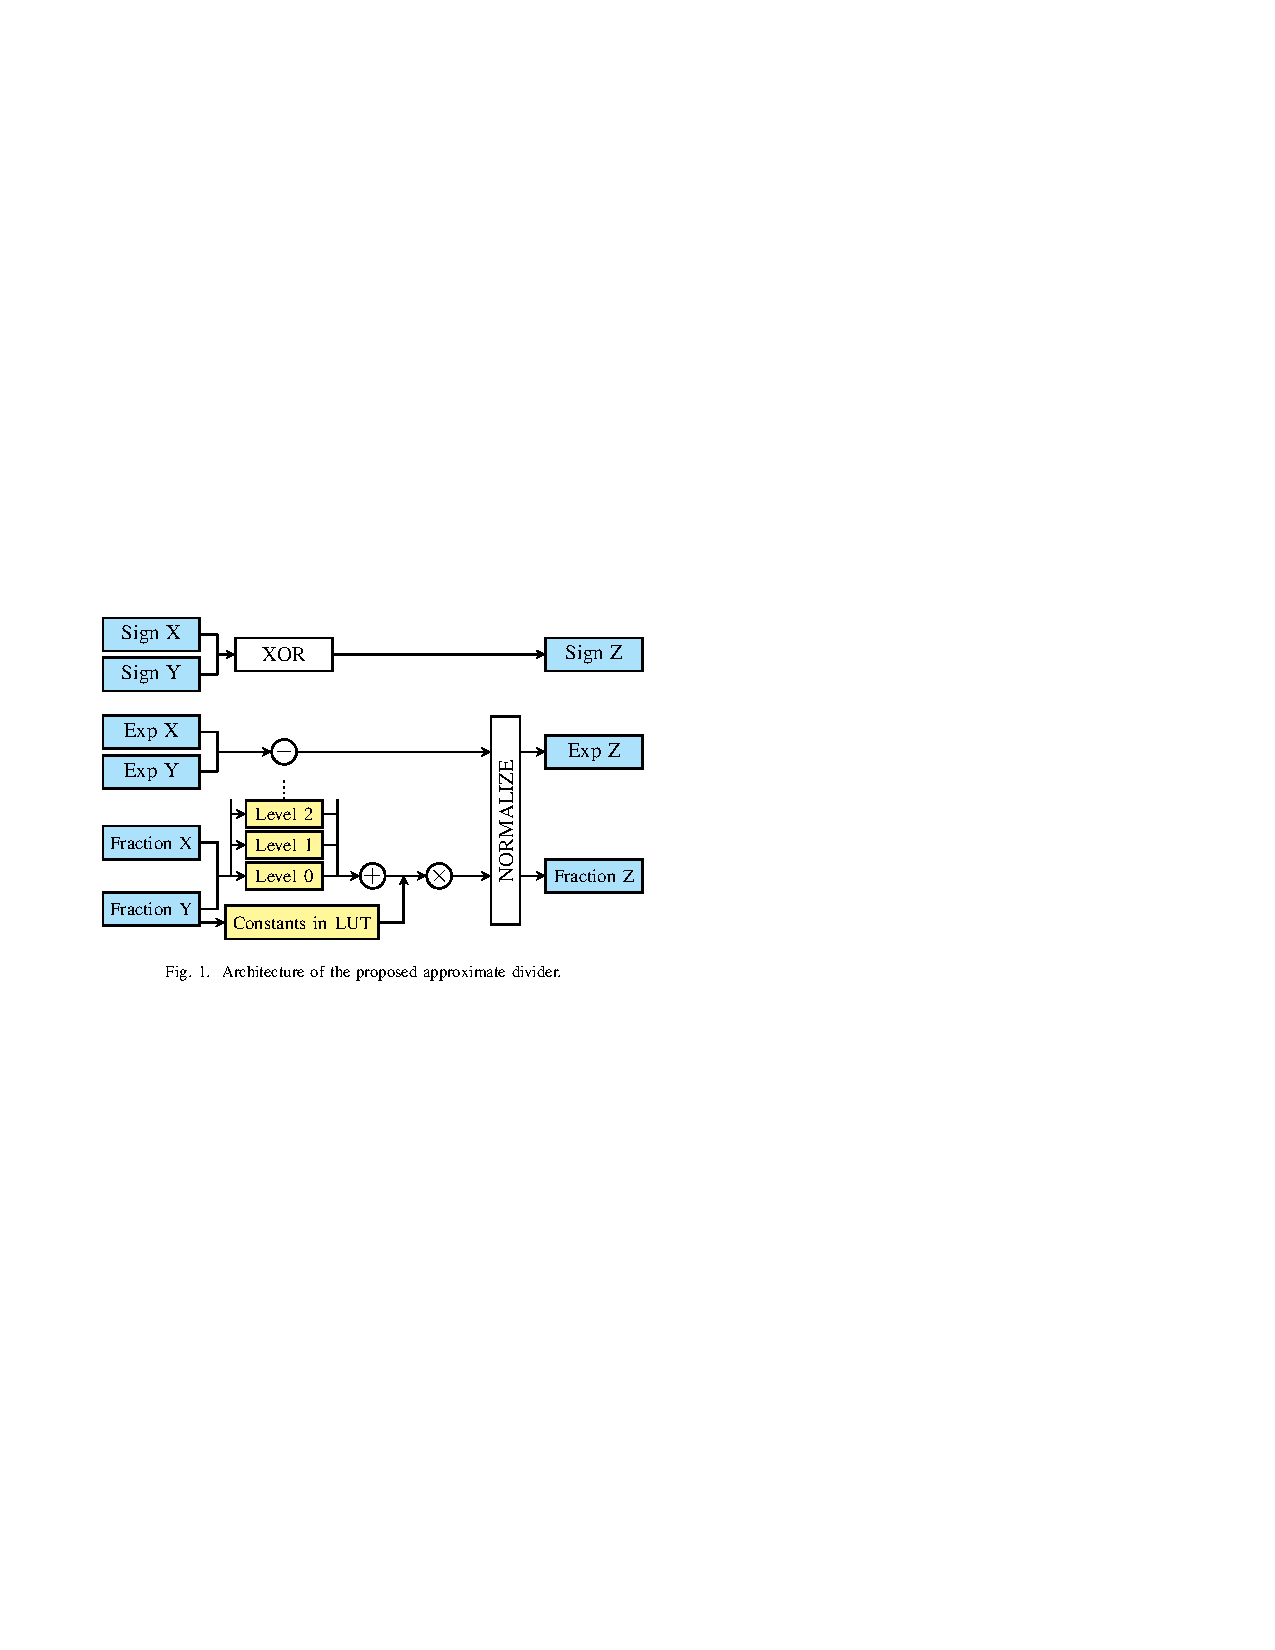
\includegraphics[width=0.99\columnwidth]{Figure 1.pdf}
 % \caption{这是PDF图片的标题}  % 图题
  \label{Figure 1}             % 引用标签（唯一）
\end{figure}

%----------------------(Figure 1)--------------------

As shown in Figure 1, level 0 is denoted as the basic approximation module, which provides an initial estimate, while the deeper levels act as error compensation to gradually improve the overall accuracy. Thus by specifying the desired depths we can realize the run-time configurability.






%----------------------(Figure 2)---------------------

\begin{figure}[h]   % h=here（优先当前位置），可用 [!h] 强制
  \centering        % 居中
  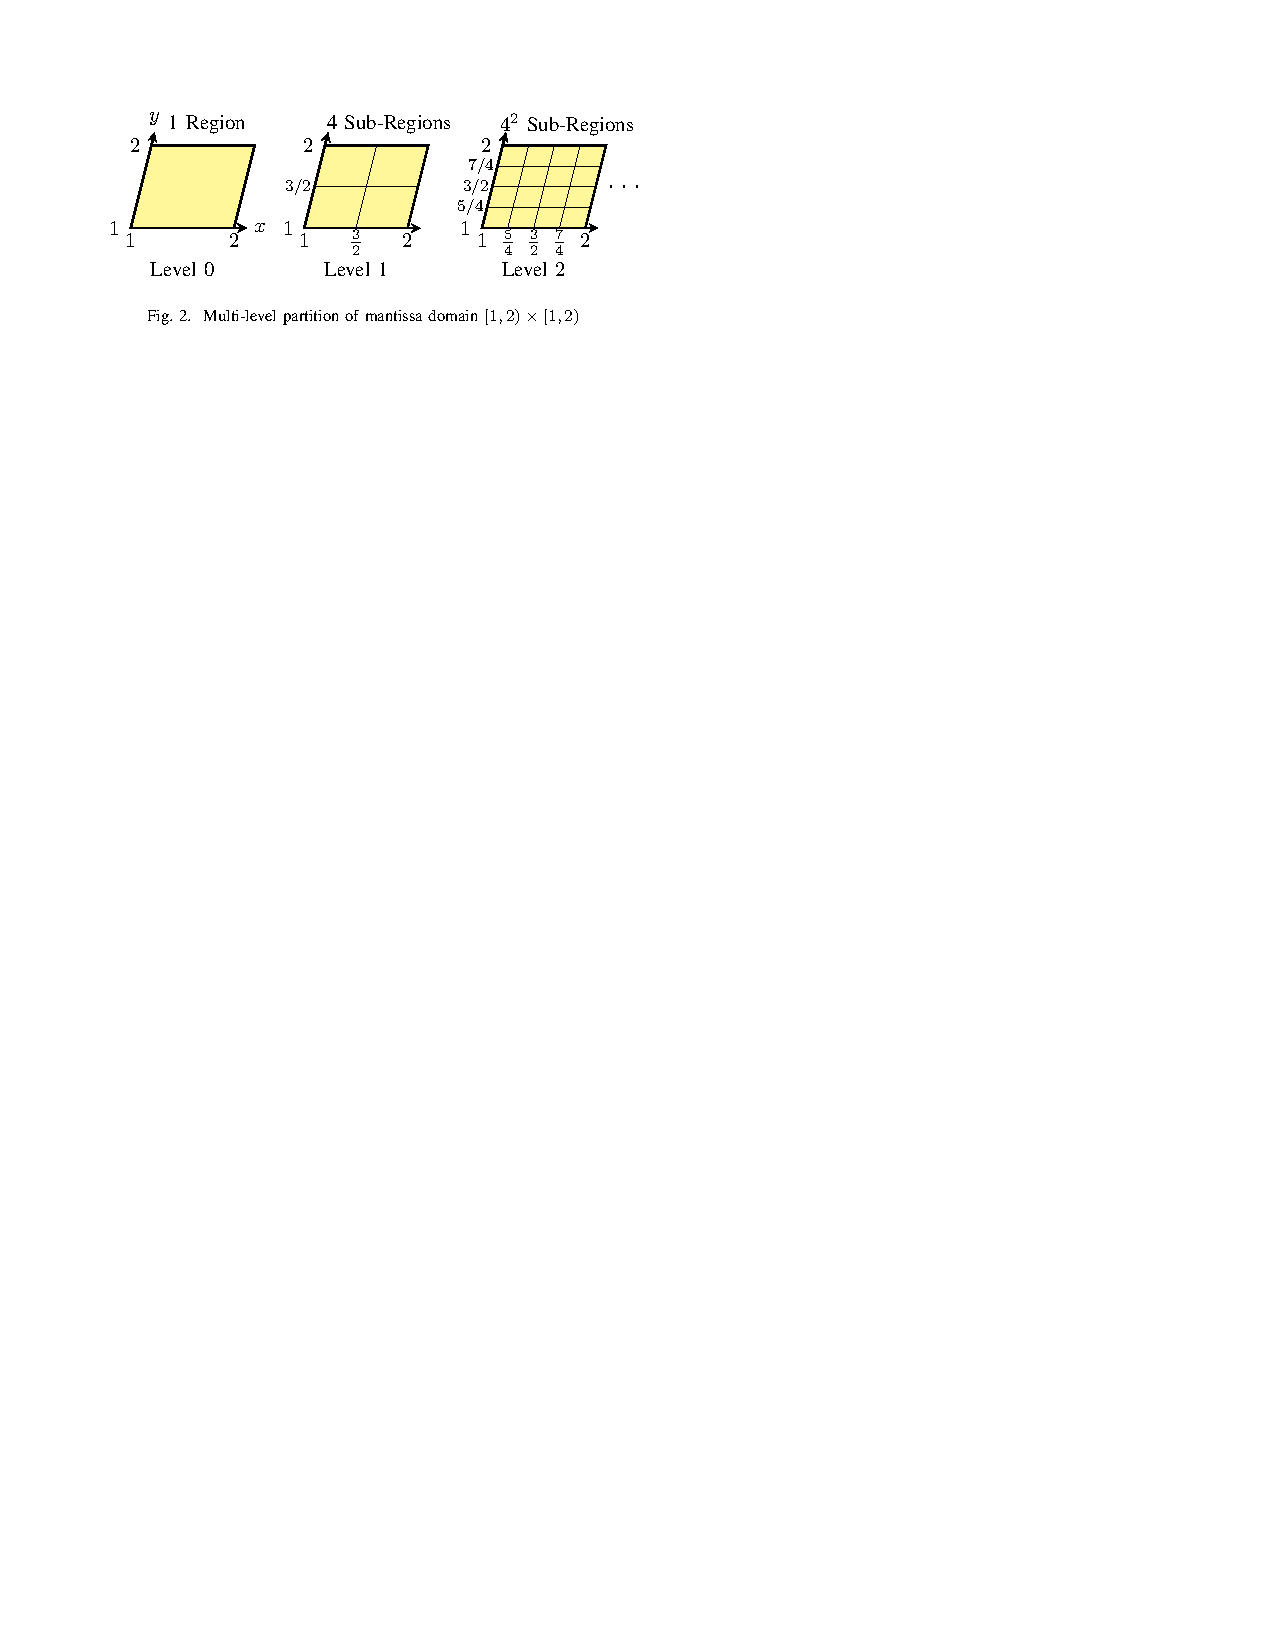
\includegraphics[width=0.995\columnwidth]{Figure 2.pdf}
 % \caption{这是PDF图片的标题}  % 图题
  \label{Figure 2}             % 引用标签（唯一）
\end{figure}
%----------------------(Figure 2)--------------------





The initial domain for the mantissas in an FP divider is $[1,2)\times [1, 2)$. For one level deeper, as shown in Figure 2 we partition each rectangle domain to $2^{2}$-subregions of rectangle shapes from the middle points as follows:

level 0: $[1,2)\times [1, 2)$;

level 1: $[1, 1.5)\times [1, 1.5),\;[1, 1.5)\times [1.5, 2),\;[1.5, 2)\times [1, 1.5),\;[1.5, 2)\times [1.5, 2)$;

level $n$: $[x_{p-1}^{n}, x_{p}^{n})\times [y_{q-1}^{n}, y_{q}^{n})$, where $x_{p}^{n}=1+{p\over 2^{n}}, y_{q}^{n}=1+{q\over 2^{n}}$.

We denote the $p$th interval for $x$ on the $n$-level as $[x_{p-1}^{n}, x_{p}^{n})$ for $p=1,\cdots,2^{n}$ and similarly the $q$th interval for $y$ on the $n$-level as
$[y_{q-1}^{n}, y_{q}^{n})$ for $q=1,\cdots,2^{n}$. Thus the interval middle points are
\begin{eqnarray}
\widehat{x_{p}^{n}}=x_{p-1}^{n}+{1\over 2^{n+1}}=1+{p-1\over 2^{n}}+{1\over 2^{n+1}}=1+{2p-1\over 2^{n+1}}=k_{2}\nonumber\\
\widehat{y_{q}^{n}}=y_{q-1}^{n}+{1\over 2^{n+1}}=1+{q-1\over 2^{n}}+{1\over 2^{n+1}}=1+{2q-1\over 2^{n+1}}=k_{1}.\nonumber
\end{eqnarray}

Therefore by equation (\ref{SecondMethod}), for any level $n$ we can derive the following:
\begin{equation}z_{D}^{n}={1\over(\widehat{y_{q(n)}^{n}})^{2}}(\widehat{x_{p(n)}^{n}}\cdot\widehat{y_{q(n)}^{n}}+\widehat{y_{q(n)}^{n}}\cdot x-\widehat{x_{p(n)}^{n}}\cdot y),\label{nlevelSecondMethod}\end{equation}
where $p(n), q(n)$ are the indexes to specify the subregion which $(x, y)$ belongs to in the $n$th level. In the following, we will implement ${1\over(\widehat{y_{q(n)}^{n}})^{2}}$
and $w_{n}=\widehat{x_{p(n)}^{n}}\cdot\widehat{y_{q(n)}^{n}}+\widehat{y_{q(n)}^{n}}\cdot x-\widehat{x_{p(n)}^{n}}\cdot y$ separately.

{\bf (i)\;\;First for  ${\boldsymbol w_{n}}$}. The following method is similar to that for approximate multiplier in \cite{CTChen}. For convenience of readers, we list main calculations of this method. We have
\begin{flalign}
w_{n} &= \widehat{x_{p(n)}^{n}}\cdot\widehat{y_{q(n)}^{n}}+\widehat{y_{q(n)}^{n}}\cdot x-\widehat{x_{p(n)}^{n}}\cdot y \nonumber\\
&= (w_{n}-w_{n-1})+(w_{n-1}-w_{n-2})+\cdots+(w_{1}-w_{0})+w_{0} \nonumber\\
&= \sum_{i=1}^{n}\triangle w_{i}+\widehat{x_{p(0)}^{0}}\cdot\widehat{y_{q(0)}^{0}}+\widehat{y_{q(0)}^{0}}\cdot x-\widehat{x_{p(0)}^{0}}\cdot y \nonumber\\
&= \sum_{i=1}^{n}\triangle w_{i}+2.25+1.5x-1.5y .\label{wn}
\end{flalign}

%------------------------(Figure 3)-------------------------

\begin{figure}[h]   % h=here（优先当前位置），可用 [!h] 强制
  \centering        % 居中
  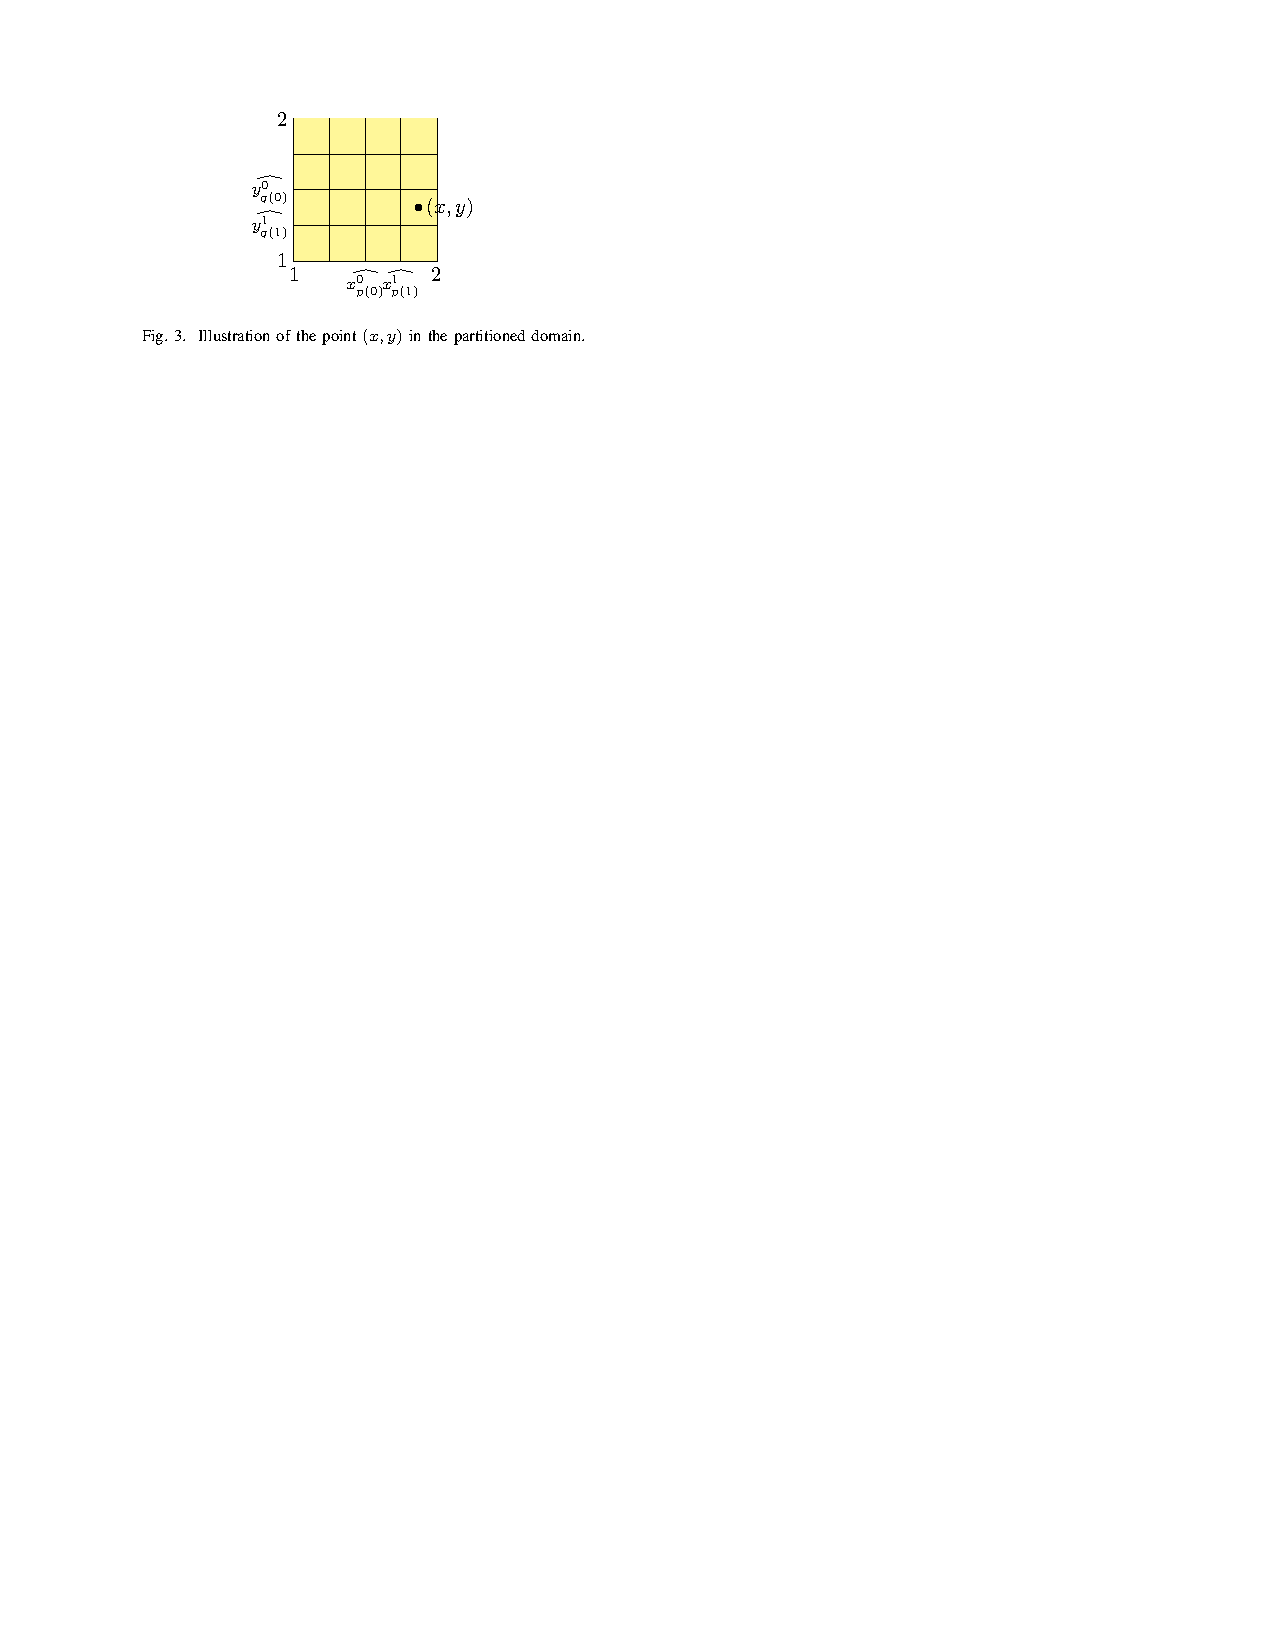
\includegraphics{Figure 3.pdf}
 % \caption{这是PDF图片的标题}  % 图题
  \label{Figure 3}             % 引用标签（唯一）
\end{figure}



%-----------------------(Figure 3)--------------------------



It is easy to calculate that
$$\widehat{x_{p(0)}^{0}}={3\over 2};$$
and
$$\widehat{x_{p(1)}^{1}}={3\over 2}+{1\over 2^{2}}\; \mbox{if}\; x>\widehat{x_{p(0)}^{0}};$$
$$\widehat{x_{p(1)}^{1}}={3\over 2}-{1\over 2^{2}}\; \mbox{if}\; x<\widehat{x_{p(0)}^{0}};$$
i.e.$$\widehat{x_{p(1)}^{1}}=\widehat{x_{p(0)}^{0}}+{x[1]?(1):(-1)\over 2^{2}}.$$

Thus in general, we have
$$\widehat{x_{p(n)}^{n}}=\widehat{x_{p(n-1)}^{n-1}}+{x[n]?(1):(-1)\over 2^{n+1}}$$
and similarly
$$\widehat{y_{q(n)}^{n}}=\widehat{y_{q(n-1)}^{n-1}}+{y[n]?(1):(-1)\over 2^{n+1}},$$
where $x[n], y[n]$ are the $n$th bit after decimal point in binary expansion of $x, y$ separately. Thus
{\small\begin{flalign}
\triangle w_{n}&=[\widehat{x_{p(n)}^{n}}\cdot\widehat{y_{q(n)}^{n}}+\widehat{y_{q(n)}^{n}}\cdot x-\widehat{x_{p(n)}^{n}}\cdot y]\nonumber\\
&-[\widehat{x_{p(n-1)}^{n-1}}\cdot\widehat{y_{q(n-1)}^{n-1}}+\widehat{y_{q(n-1)}^{n-1}}\cdot x-\widehat{x_{p(n-1)}^{n-1}}\cdot y]\nonumber\\
&=[\widehat{x_{p(n)}^{n}}\cdot\widehat{y_{q(n)}^{n}}-\widehat{x_{p(n-1)}^{n-1}}\cdot\widehat{y_{q(n-1)}^{n-1}}]\nonumber\\
&+(\widehat{y_{q(n)}^{n}}-\widehat{y_{q(n-1)}^{n-1}})x-(\widehat{x_{p(n)}^{n}}-\widehat{x_{p(n-1)}^{n-1}})y\nonumber\\
&=[(\widehat{x_{p(n-1)}^{n-1}}+{x[n]?(1):(-1)\over 2^{n+1}})\cdot(\widehat{y_{q(n-1)}^{n-1}}+{y[n]?(1):(-1)\over 2^{n+1}})\nonumber\\
&-\widehat{x_{p(n-1)}^{n-1}}\cdot\widehat{y_{q(n-1)}^{n-1}}]\nonumber\\
&+{y[n]?(1):(-1)\over 2^{n+1}}x-{x[n]?(1):(-1)\over 2^{n+1}}y\nonumber\\
&=(x+\widehat{x_{p(n-1)}^{n-1}})\cdot{y[n]?(1):(-1)\over 2^{n+1}}\nonumber\\
&+(\widehat{y_{q(n-1)}^{n-1}}-y)\cdot{x[n]?(1):(-1)\over 2^{n+1}}\nonumber\\
&+{x[n]?(1):(-1)\over 2^{n+1}}\cdot{y[n]?(1):(-1)\over 2^{n+1}}\nonumber\\
&=(x+\widehat{x_{p(n-1)}^{n-1}})\cdot(y[n]?(1):(-1))>>n+1\nonumber\\
&+(\widehat{y_{q(n-1)}^{n-1}}-y)\cdot(x[n]?(1):(-1))>>n+1\nonumber\\
&+(x[n]^{\wedge} y[n])?(-1):(1)>>2n+2.\label{deltawn}
\end{flalign}}


Note that $\widehat{x_{p(n-1)}^{n-1}}, \widehat{y_{q(n-1)}^{n-1}}$ are the middle points of the intervals that contain $x, y$ separately.
$(x+\widehat{x_{p(n-1)}^{n-1}})\cdot(y[n]?(1):(-1))>>n+1$ can be implemented in circuit with 1 addition operation, at most 1 inversion operation and 1 $(n+1)$-bits right shift operation;
$(\widehat{y_{q(n-1)}^{n-1}}-y)\cdot(x[n]?(1):(-1))>>n+1$ can be implemented in circuit with logic operations by turning the first $n$ bits in $y$ to 0 and bit flipping (if necessary) for the rest of bits in $y$, at most 1 inversion operation and 1 $(n+1)$-bits right shift operation; and
$(x[n]^{\wedge} y[n])?(-1):(1)>>2n+2$
 can be implemented with 1 XOR operation, at most 1 inversion operation and 1 $(2n+2)$-bits right shift operation.

{\bf (ii)\;\; Secondly for ${\boldsymbol {1\over(\widehat{y_{q(n)}^{n}})^{2}}}$}. ${1\over(\widehat{y_{q(n)}^{n}})^{2}}$ is constant that can be pre-calculated and pre-loaded lookup tables for each level $n$ and $q(n)=1, 2,\cdots, 2^{n}$. Since $$\begin{array}{rcl}
\widehat{y_{q(n)}^{n}}&=&\widehat{y_{q(n-1)}^{n-1}}+\frac{y[n]?1:(-1)}{2^{n+1}}\\
&=&\widehat{y_{q(n-2)}^{n-2}}+\frac{y[n-1]?1:(-1)}{2^{n}}+\frac{y[n]?1:(-1)}{2^{n+1}}\\
&=&\cdots=\widehat{y_{q(0)}^{0}}+\sum\limits_{k=1}^{n}\frac{y[k]?1:(-1)}{2^{k+1}}
\end{array},$$
we list the constants $\frac{1}{(\widehat{y^{n}_{q(n)}})^2}$ for level $0,1,2,3$ as follows:

\begin{align*}
\text{level }0:\quad & \frac{1}{(\widehat{y^{0}_{q(0)}})^2} = \frac1{(3/2)^2}\\[6pt]
\text{level }1:\quad & \frac{1}{(\widehat{y^{1}_{q(1)}})^2} =
\begin{cases}
\frac1{(7/4)^2} & \text{if }y[1]=1;\\[4pt]
\frac1{(5/4)^2} & \text{if }y[1]=0;
\end{cases}\\[12pt]
\text{level }2:\quad & \frac{1}{(\widehat{y^{2}_{q(2)}})^2}  =
\begin{cases}
\frac1{(15/8)^2} & y[1]=1,\;y[2]=1;\\[4pt]
\frac1{(13/8)^2} & y[1]=1,\;y[2]=0;\\[4pt]
\frac1{(11/8)^2}  & y[1]=0,\;y[2]=1;\\[4pt]
\frac1{(9/8)^2} & y[1]=0,\;y[2]=0;
\end{cases}\\[18pt]
\text{level }3:\quad & \frac{1}{(\widehat{y^{3}_{q(3)}})^2}  =
\begin{cases}
\frac1{(31/16)^2}  & y[1]=1,y[2]=1,y[3]=1;\\[3pt]
\frac1{(29/16)^2}  & y[1]=1,y[2]=1,y[3]=0;\\[3pt]
\frac1{(27/16)^2}  & y[1]=1,y[2]=0,y[3]=1;\\[3pt]
\frac1{(25/16)^2}  & y[1]=1,y[2]=0,y[3]=0;\\[3pt]
\frac1{(23/16)^2}  & y[1]=0,y[2]=1,y[3]=1;\\[3pt]
\frac1{(21/16)^2}  & y[1]=0,y[2]=1,y[3]=0;\\[3pt]
\frac1{(19/16)^2}  & y[1]=0,y[2]=0,y[3]=1;\\[3pt]
\frac1{(17/16)^2}  & y[1]=0,y[2]=0,y[3]=0;
\end{cases}
\end{align*}
%------------------------(Figure 4)-------------------------

\begin{figure}[h]   % h=here（优先当前位置），可用 [!h] 强制
  \centering        % 居中
  
\includegraphics{Figure 4.pdf}
 % \caption{这是PDF图片的标题}  % 图题
  \label{Figure 4}             % 引用标签（唯一）
\end{figure}



%-----------------------(Figure 4)--------------------------

For example, mantissa $y=\overline{1.1\,0\,1\,0\,1\cdots}$ (see Figure 4), 
we have
$$\begin{array}{rcl}
\frac1{(\widehat{y^{0}_{q(0)}})^2} &= &\frac1{(3/2)^2},\\[3pt]
\frac1{(\widehat{y^{1}_{q(1)}})^2} &= &\frac1{\bigl(\frac32+\frac14\bigr)^2} = \frac1{(7/4)^2},\\[3pt]
\frac1{(\widehat{y^{2}_{q(2)}})^2}&= &\frac1{\bigl(\frac32+\frac14-\frac18\bigr)^2} = \frac1{(13/8)^2},\\[3pt]
\frac1{(\widehat{y^{3}_{q(3)}})^2} &= &\frac1{\bigl(\frac32+\frac14-\frac18+\frac1{16}\bigr)^2} = \frac1{(27/16)^2},\\[3pt]
\frac1{(\widehat{y^{4}_{q(4)}})^2} &= &\frac1{\bigl(\frac32+\frac14-\frac18+\frac1{16}-\frac1{32}\bigr)^2} = \frac1{(53/32)^2}.
\end{array}$$

\subsection{\small{Architecture for Multi-Level Approximate Divider-Multiplier}}
\label{ArchDM}

It follows from \cite{CTChen} that for any level $n$ we have the following:
\begin{flalign}
z_{M}^{n} &= -\widehat{x_{p(n)}^{n}}\cdot\widehat{y_{q(n)}^{n}}+\widehat{y_{q(n)}^{n}}\cdot x+\widehat{x_{p(n)}^{n}}\cdot y \nonumber\\
&= \sum_{i=1}^{n}\triangle z_{i}-\widehat{x_{p(0)}^{0}}\cdot\widehat{y_{q(0)}^{0}}+\widehat{y_{q(0)}^{0}}\cdot x+\widehat{x_{p(0)}^{0}}\cdot y \nonumber\\
&= \sum_{i=1}^{n}\triangle z_{i}-2.25+1.5x+1.5y, \label{zn}
\end{flalign}
where 
{\small\begin{flalign}
\triangle z_{n}&=[-\widehat{x_{p(n)}^{n}}\cdot\widehat{y_{q(n)}^{n}}+\widehat{y_{q(n)}^{n}}\cdot x+\widehat{x_{p(n)}^{n}}\cdot y]\nonumber\\
&-[-\widehat{x_{p(n-1)}^{n-1}}\cdot\widehat{y_{q(n-1)}^{n-1}}+\widehat{y_{q(n-1)}^{n-1}}\cdot x+\widehat{x_{p(n-1)}^{n-1}}\cdot y]\nonumber\\
&=(x-\widehat{x_{p(n-1)}^{n-1}})\cdot(y[n]?(1):(-1))>>n+1\nonumber\\
&+(y-\widehat{y_{q(n-1)}^{n-1}})\cdot(x[n]?(1):(-1))>>n+1\nonumber\\
&+(x[n]^{\wedge} y[n])?(1):(-1)>>2n+2.\label{deltazn}
\end{flalign}}
As mentioned in \cite{CTChen}, $(x-\widehat{x_{p(n-1)}^{n-1}})\cdot(y[n]?(1):(-1))>>n+1$ and
$(y-\widehat{y_{q(n-1)}^{n-1}})\cdot(x[n]?(1):(-1))>>n+1$ can be implemented in circuit with logic operations by turning the first $n$ bits in $x, y$ to 0 and bit flipping (if necessary) for the rest of bits in $x, y$, at most 1 inversion operation and 1 $(n+1)$-bits right shift operation; and
$(x[n]^{\wedge} y[n])?(1):(-1)>>2n+2$
 can be implemented with 1 XOR operation, at most 1 inversion operation and 1 $(2n+2)$-bits right shift operation.


Comparing Eqs. (\ref{deltawn}) with (\ref{deltazn}), we arrive at the following relations: 
\begin{flalign}
\triangle w_{n} &=-\triangle z_{n}+2x\cdot(y[n]?(1):(-1))>>n+1\label{d_m_1}\\ 
w_{0}&=-z_{M}^{0}+3x,\label{d_m_2}
\end{flalign}
where $w_{0}=2.25+1.5x-1.5y$ and $z_{M}^{0}=-2.25+1.5x+1.5y;$
and 
{\small\begin{flalign}
&(x\pm\widehat{x_{p(n-1)}^{n-1}})\cdot(y[n]?(1):(-1))>>n+1\nonumber\\
&\mp[(y-\widehat{y_{q(n-1)}^{n-1}})\cdot(x[n]?(1):(-1))>>n+1\nonumber\\
&+(x[n]^{\wedge} y[n])?(1):(-1)>>2n+2]=
\begin{cases}
\triangle w_{n};\\
\triangle z_{n};
\end{cases}
\label{d_m_3}
\end{flalign}}

\begin{flalign}
1.5x\mp(1.5y-2.25)=
\begin{cases}
w_{0};\\
z_{M}^{0}.
\end{cases}\label{d_m_4}
\end{flalign}

Motivated by the similarity between $z_{M}^{n}$ and the main part $w_{n}$ of $z_{D}^{n}$, we propose a unified hardware architecture supporting both approximate floating-point division and multiplication as shown in Figure 5.

%------------------------(Figure 5)-------------------------

\begin{figure}[h]   % h=here（优先当前位置），可用 [!h] 强制
  \centering        % 居中
  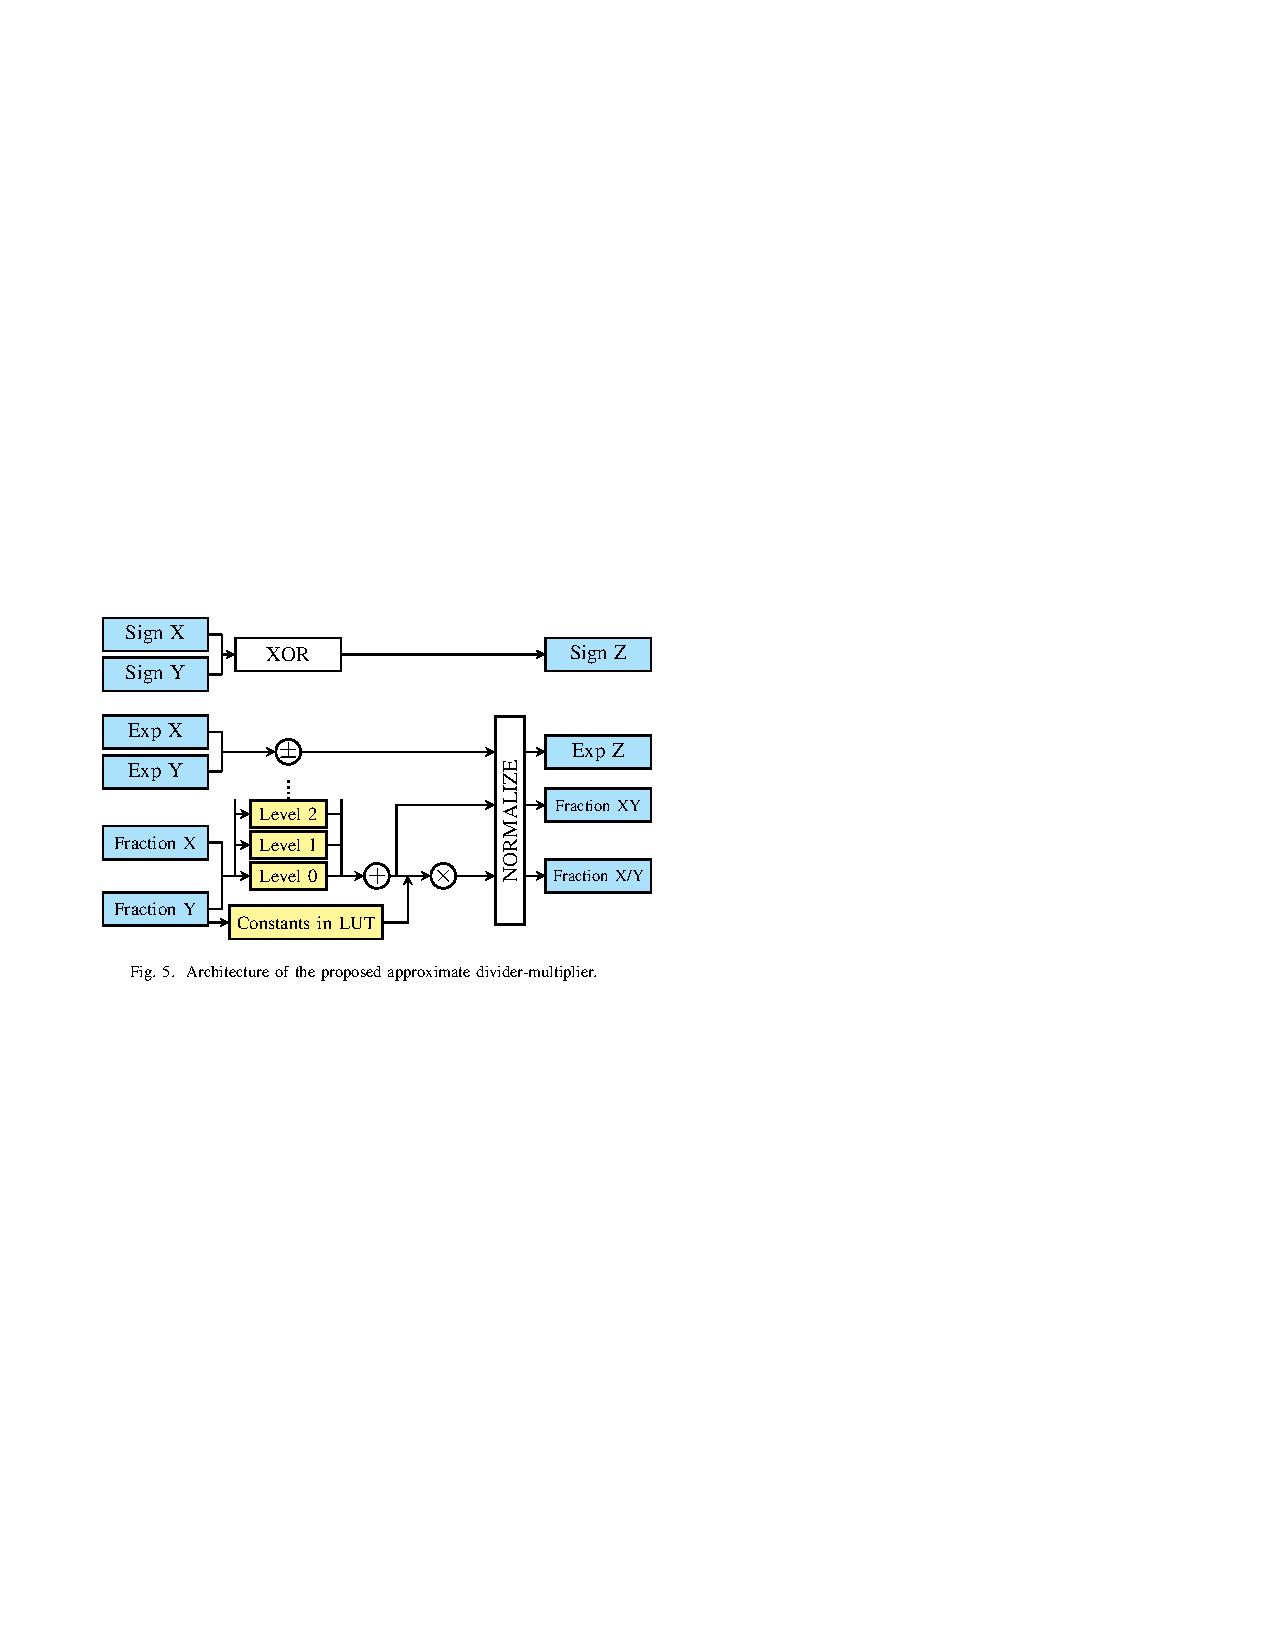
\includegraphics{Figure 5.pdf}
 % \caption{这是PDF图片的标题}  % 图题
  \label{Figure 5}             % 引用标签（唯一）
\end{figure}


\section{ERROR ANALYSIS}
\label{ErrAna4}
In this section, we further discuss the absolute error for different levels of approximations in the proposed divider. We recall the Taylor's Theorem for two variables: for $0<\theta<1$,
$$\begin{array}{l}
f(x,y)=f(x_{0}, y_{0})+[(x-x_{0}){\partial\over\partial x}+(y-y_{0}){\partial\over\partial y}]f(x_{0}, y_{0})\\
+[(x-x_{0}){\partial\over\partial x}+(y-y_{0}){\partial\over\partial y}]^{2}f(x_{0}+\theta(x-x_{0}), y_{0}+\theta(y-y_{0})).
\end{array}$$

For $f(x, y)={x\over y}$ on $[x_{1}, x_{2}]\times [y_{1}, y_{2}]$ and $x_{0}={x_{1}+x_{2}\over 2}=k_{2}, y_{0}={y_{1}+y_{2}\over 2}=k_{1}$ as the symbols in Section \ref{AppDivider3}, we have
{\small\begin{flalign}
{x\over y}&={x_{0}\over y_{0}}+(x-x_{0})\cdot{1\over y_{0}}+(y-y_{0})\cdot(-{x_{0}\over y_{0}^{2}})\nonumber\\
&+{1\over 2}[(x-x_{0})^{2}\cdot 0+2(x-x_{0})(y-y_{0})(-{1\over(y_{0}+\theta(y-y_{0}))^{2}})\nonumber\\
&+(y-y_{0})^{2}\cdot{2(x_{0}+\theta(x-x_{0}))\over(y_{0}+\theta(y-y_{0}))^{3}}]\nonumber\\
&={1\over k_{1}^{2}}(k_{1}k_{2}+k_{1}x-k_{2}y)\label{TaylorResult}\\
&+{(y-y_{0})[(y-y_{0})(x_{0}+\theta(x-x_{0}))-(x-x_{0})(y_{0}+\theta(y-y_{0}))]\over(y_{0}+\theta(y-y_{0}))^{3}}.\nonumber\end{flalign}}

It follows from equation (\ref{SecondMethod}) and (\ref{TaylorResult}) that
$${x\over y}=z_{D}+err, \;\mbox{for}\; (x, y)\in [x_{1}, x_{2}]\times [y_{1}, y_{2}],$$
where $err$ is  {\footnotesize \begin{equation}{(y-y_{0})[(y-y_{0})(x_{0}+\theta(x-x_{0}))-(x-x_{0})(y_{0}+\theta(y-y_{0}))]\over(y_{0}+\theta(y-y_{0}))^{3}}.\label{TaylorErr}\end{equation}}

Thus for the $n$th level and $(x, y)\in[x_{p(n)-1}^{n}, x_{p(n)}^{n})\times [y_{q(n)-1}^{n}, y_{q(n)}^{n})$, where $x_{p(n)}^{n}=1+{p(n)\over 2^{n}}$ and $y_{q(n)}^{n}=1+{q(n)\over 2^{n}}$, it follows from the equation (\ref{TaylorErr}) that
{\small\begin{flalign}|err|&\leq {|y-y_{0}|(2|y-y_{0}|+2|x-x_{0}|)\over 1^{3}}\nonumber\\
&\leq {1\over 2^{n+1}}\cdot{4\over 2^{n+1}}={1\over 4^{n}}.\label{AbsTaylorErr}\end{flalign}}

%----------------------(Figure 6-7)---------------------

\begin{figure}[h]
\centering
% 0.95倍单栏宽度，刚好适配IEEE双栏，自动等比缩小
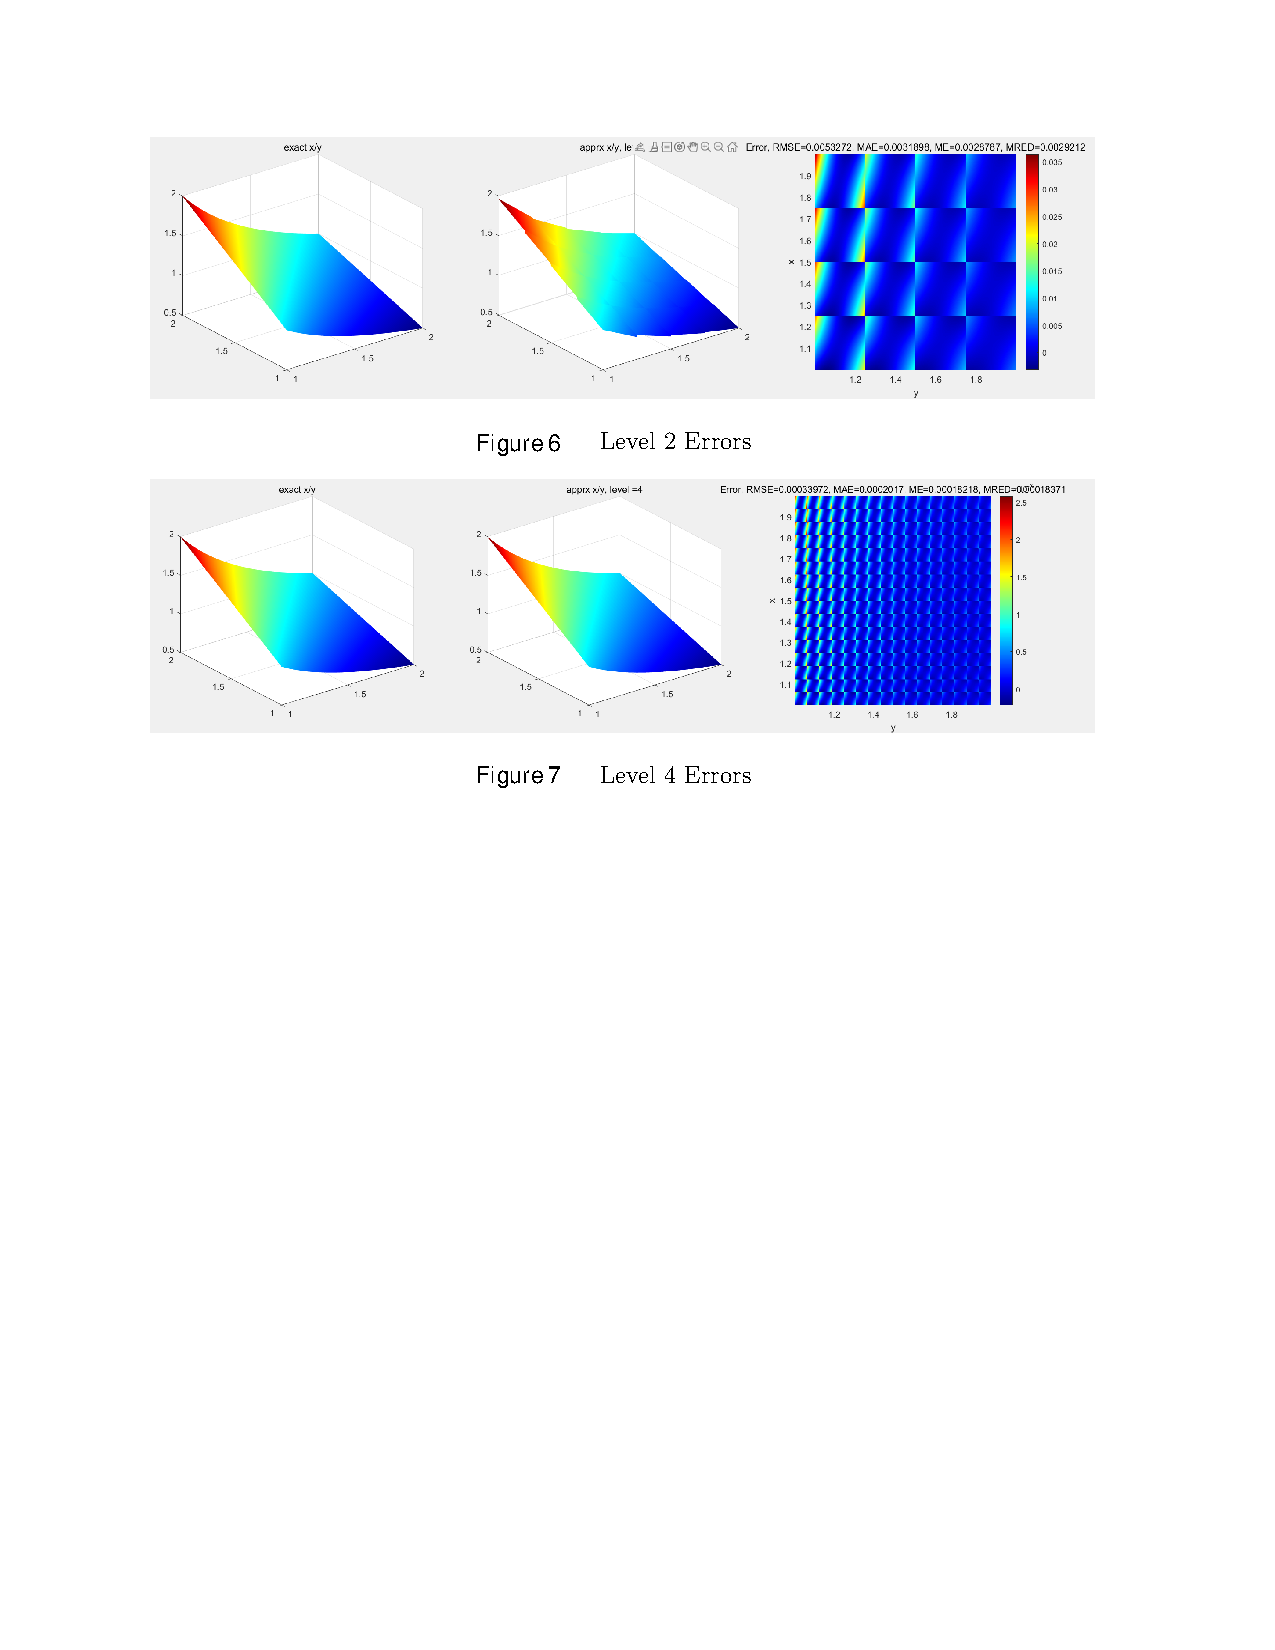
\includegraphics[width=0.95\columnwidth]{Figure 6.pdf}
%\caption{Level Errors.}
\label{Figure 6}
\end{figure}
%----------------------(Figure 6-7)---------------------



\section{EXPERIMENTAL RESULTS}
\label{Experiment5}
\subsection{Circuit Implementation for Multi-Level}
\label{Circuit5.1}
For $x, y \in [1,2)$, it follows from Equatoins (\ref{nlevelSecondMethod}), (\ref{wn}), (\ref{zn}), (\ref{d_m_3}) and (\ref{d_m_4}) that

\begin{align*}
\text{level }0:\quad & \frac{x}{y}\approx z_{D}^{0}=\frac1{(\widehat{y^{0}_{q(0)}})^2} w_{0};\\[3pt]
&xy\approx z_{M}^{0};\\[3pt]
\text{level }1:\quad & \frac{x}{y}\approx z_{D}^{1}=\frac{1}{(\widehat{y^{1}_{q(1)}})^2} (\triangle w_{1}+w_{0});\\[3pt]
&xy\approx z_{M}^{1}=\triangle z_{1}+z_{M}^{0};\\[3pt]
\text{level }2:\quad & \frac{x}{y}\approx z_{D}^{2}=\frac{1}{(\widehat{y^{2}_{q(2)}})^2} (\triangle w_{2}+\triangle w_{1}+w_{0});\\[3pt]
&xy\approx z_{M}^{2}=\triangle z_{2}+\triangle z_{1}+z^{0}_{M};\\[3pt]
\cdots\cdots&\\[3pt]
\end{align*}
where 
\begin{align*}
w_{0} \;\text{or}\; z_{M}^{0}&=1.5x\mp(1.5y-2.25);\nonumber\\[3pt]
\triangle w_{1}\;\text{or}\;\triangle z_{1}&=(x\pm\widehat{x_{p(0)}^{0}})\cdot(y[1]?(1):(-1))>>2\nonumber\\[3pt]
&\mp[(y-\widehat{y_{q(0)}^{0}})\cdot(x[1]?(1):(-1))>>2\nonumber\\[3pt]
&+(x[1]\text{\textasciicircum} y[1]?(1):(-1))>>4];\nonumber\\[3pt]
\triangle w_{2}\;\text{or}\;\triangle z_{2}&=(x\pm\widehat{x_{p(1)}^{1}})\cdot(y[2]?(1):(-1))>>3\nonumber\\[3pt]
&\mp[(y-\widehat{y_{q(1)}^{1}})\cdot(x[2]?(1):(-1))>>3\nonumber\\[3pt]
&+(x[2]\text{\textasciicircum} y[2]?(1):(-1))>>6];\nonumber\\[3pt]
\cdots\cdots&\nonumber\\[3pt]
\end{align*}

This section further presents a concrete multi-level architecture designed to implement these
algorithms (divide or multiple) for $x, y\in [1, 2)$, allowing for dynamic configuration at run-time, which is illustrated in Figure 8. The circuit implementation of 
\(\triangle w_n,  \triangle z_{n}\) is detailed in subsection \ref{ArchMulti3.4} and \ref{ArchDM}. The proposed approximate divider organically combines the multi-level architecture with the LUT-based design.



%----------------------(Figure 8)---------------------

\begin{figure}[h]   % h=here（优先当前位置），可用 [!h] 强制
  \centering        % 居中
  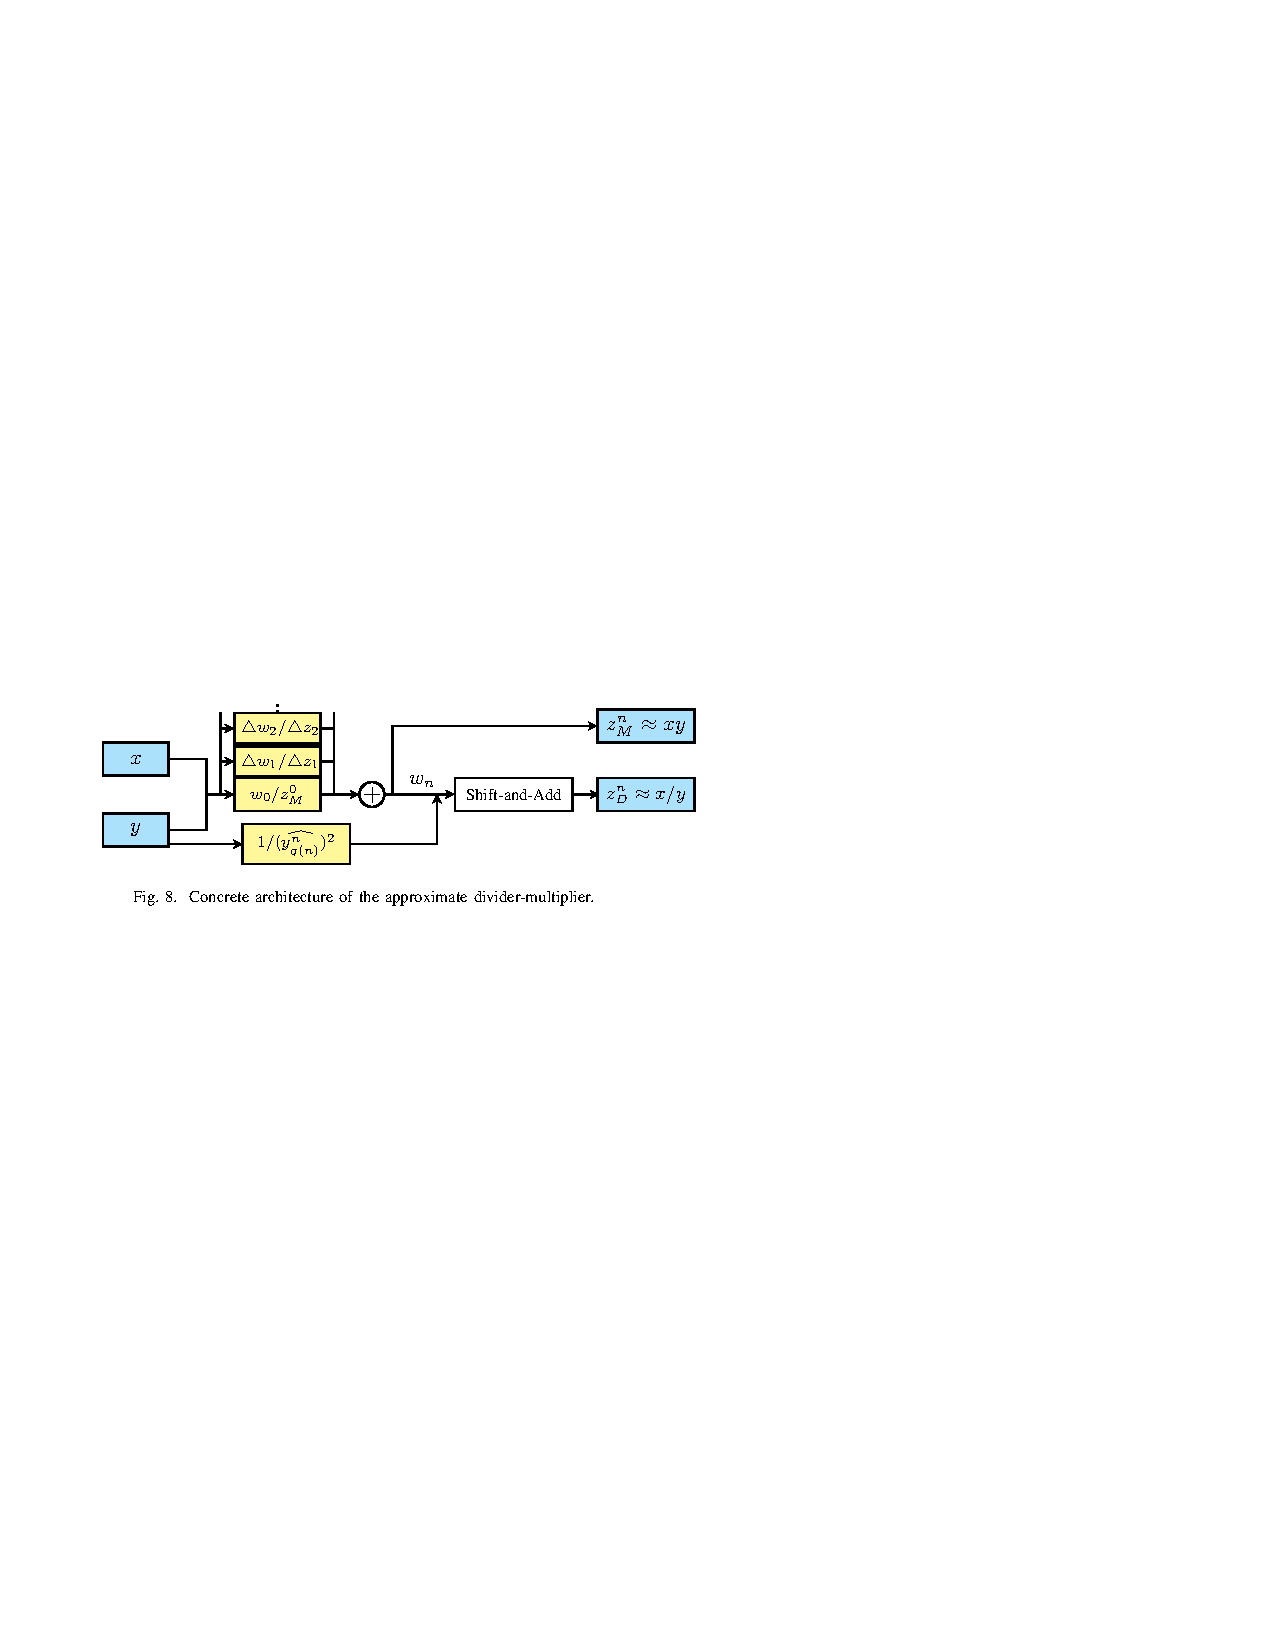
\includegraphics[width=0.99\columnwidth]{Figure 8.pdf}
 % \caption{这是PDF图片的标题}  % 图题
  \label{Figure 8}             % 引用标签（唯一）
\end{figure}

%----------------------(Figure 8)--------------------

\section{APPLICATIONS}
\label{Application6}

We evaluated the proposed divider across different approximate levels, focusing on accuracy, resource utilization,
and performance. This section is dedicated to examining the disparities between the outcomes of the proposed approximate divider 
and the exact divider in practical applications. We conduct several benchmark tests, include image processing approaches
such as change detection, background removal, K-Mean image color quantization, and Softmax layers in neural networks.

\section{CONCLUSIONS}
\label{Conlusion7}
In this work, we proposed a design for multi-level approximate FP divider with runtime configurability. The architecture can reach the optimal approximation and unbiased error distribution easily without increasing much area and delay overhead.

\begin{thebibliography}{999}
\bibitem{CTChen} C.T. Chen, et al., ``Optimally Approximated and Unbiased Floating Point Multiplier with Runtime Configurability,"  International Conference on Computer-Aided Design (ICCAD), pp.1-9, 2020.
\bibitem{JHan} J. Han and M. Orshansky, ``Approximate Computing: An Emerging Paradigm for Energy-Efficient Design," European Test Symposium(ETS), pp.1-6, 2013.
\bibitem{VGupta2011} V. Gupta, et al., ``IMPACT: IMPrecise Adders for Low-Power Approximate Computing," International Symposium on Low Power Electronics and Design (ISLPED), pp. 409-414,2011.
\bibitem{VGupta2013} V. Gupta, D. Mohapatra, A. Raghunathan, and K. Roy, ``Low-power digital signal processing using approximate adders," IEEE Transactions on Computer-Aided Design of Integrated Circuits and Systems, vol.32, no. 1, pp.124-137, 2013.
\bibitem{SHashemi2015}S. Hashemi, R. I. Bahar, and S. Reda, ``Drum: A dynamic range unbiased multiplier for approximate applications," International Conference on Computer-Aided Design(ICCAD), pp.418-425, 2015.
\bibitem{HMahdiani2010}H. Mahdiani, A Ahmadi, S. Fakhraie, and C. Lucas, ``Bio-inspired imprecise computational blocks for efficient VLSI implementation of soft-computing applications," IEEE Transactions on Circuits and Systems I, vol.57, no.4, pp.850-862, 2010.
\bibitem{HSaadat1} H. Saadat et al., ``Approximate Integer and Floating-Point Dividers with Near-Zero Error Bias," Design Automation Conference (DAC), pp.1-6 , 2019.
\bibitem{LChen}L. Chen et al., ``Design of Approximate Unsigned Integer Non-restoring Divider for Inexact Computing,"  Great Lakes Symposium on VLSI (GLSVLSI), pp.51-56, 2015.
\bibitem{SHashemi3} S. Hashemi et al., ``A low-power dynamic divider for approximate applications," Design Automation Conference (DAC), pp.1-6,2016.
\bibitem{HJiang9} H. Jiang et al., ``Low-Power Unsigned Divider and Square Root Circuit Designs Using Adaptive Approximation," IEEE Trans.on Computers, vol.68, no.11, pp.1635-1646, 2019.
\bibitem{MImani4}M.Imani et al., ``CADE: Configurable Approximate Divider for Energy Efficiency," Design, Automation, Test in Europe Conference and Exhibition (DATE), pp.586-589, 2019.
\bibitem{OGRatnaparkhi5}O.G. Ratnaparkhi et al., ``LEAD: Logarithmic Exponent Approximate Divider For Image Quantization Application,"	Great Lakes Symposium on VLSI (GLSVLSI), pp.437-442, 2022.
\bibitem{JMelchert2}J. Melchert et al., ``SAADI-EC: A Quality-Configurable Approximate Divider for Energy Efficiency,"	IEEE Transactions on Very Large Scale Integration (VLSI) Systems, Vol.27, no.11, pp.2680-2682, 2019.
\bibitem{JOelund6}J. Oelund et al., ``ILAFD: Accuracy-Configurable Floating-Point Divider Using an Approximate Reciprocal and an Iterative Logarithmic Multiplier," Great Lakes Symposium on VLSI (GLSVLSI), pp.639-644, 2023.
\bibitem{Bhargav}K.J.N.S. Bhargav et al., ``A newton raphson method based approximate divider design for color quantization application," in ISOCC'21, pp115-116.
\bibitem{CWen}C. Wen et al., ``PACE: A Piece-Wise Approximate and Configurable Floating-Point Divider for Energy-Efficient Computing," in DATE'2024.
\bibitem{HLiu} H. Liu et al., ``QIAD: A quadratic interpolation approximate divider," IEICE Electronics Express, vol.20, no.11, pp.1-6, 2023.
\bibitem{LWu15}L. Wu et al., ``A curve fitting approach for non-iterative divider design with accuracy and performance trade-off," International New Circuits and Systems Conference (NEWCAS), pp.1-4, 2015.
\bibitem{CWu} C. Wu et al., ``Area-Delay-Energy-Efficient Approximate Dividers Based on Piecewise Linear Fitting of Surface," IEEE Transactions on Circuits and Systems, vol. 71, no. 11, pp. 5017-5029, 2024.   
\bibitem{Ieee} IEEE Standard for Floating-Point Arithmetic, IEEE Standard 754-2008, pp. 1-70, 2008.
\bibitem{Wiki} $https://en.wikipedia.org/wiki/Division_algorithm$

\end{thebibliography}

\end{document}
